\documentclass{beamer}

\usetheme{Malmoe}
\usecolortheme{spruce}

\usepackage{amsmath,amsthm,amssymb}
\usepackage{mathtools}
\usepackage{mathrsfs}
\usepackage{enumitem}
\usepackage{physics}
\usepackage{slashed}

%Information to be included in the title page:
\title{QCD Scattering Amplitudes}
\author{Sean Ericson}
\institute{UO}
\date{June 5, 2023}
\titlegraphic{
\includegraphics[scale=0.75]{seal.jpg}}

\begin{document}

\frame{\titlepage}

\begin{frame}
    \frametitle{Nonabelian Gauge Theory}
    \alert{Introduction}
    \begin{itemize}
        \item[\textbullet]<2-> Consider a lagrangian of $N$ fields $\mathcal{L}(\phi_i)$ which is invariant under the global $SU(N)$ transformation $\phi_i \to U_{ij}\phi_j$.
        \item[\textbullet]<3-> This necessitates the inclusion of an $SU(N)$ \textit{gauge field} $A_\mu(x)$ (an $NxN$ traceless hermitian matrix field).
        \item[\textbullet]<4-> Also, we must promote normal derivatives $\partial_\mu$ to \textit{covariant derivatives} $D_\mu = \partial_\mu - igA_\mu$. 
    \end{itemize}
\end{frame}

\begin{frame}
    \frametitle{Nonabelian Gauge Theory (cont.)}
    \alert{$SU(N)$ Generators}
    \begin{itemize}
        \item[\textbullet]<2-> Gauge transformations are built from the \textit{generator matrices} $T^a$ of the symmetry group.
        \item[\textbullet]<3-> The $T^a$ satisfy the commutation relation \[ \comm{T^a}{T^b} = if^{abc}T^c \] and are normalized according to \[ \Tr[T^aT^b] = \frac{1}{2}\delta^{ab} \]
        \item[\textbullet]<4-> The gauge field can be expanded in the basis of the generators: \[ A_\mu(x) = A_\mu^a(x)T^a \] where \[ A_\mu^a(x) = 2\Tr[A_\mu(x)T^a] \]
    \end{itemize}
\end{frame}

\begin{frame}
    \frametitle{Nonabelian Gauge Theory (cont.)}
    \alert{Building the lagrangian}
    \begin{itemize}
        \item[\textbullet]<2-> The field strength is given by
        \begin{align*}
            F_{\mu\nu} &\coloneqq \frac{i}{g}\comm{D_\mu}{D_\nu} \\
            &= \partial_\mu A_\nu - \partial_\nu A_\mu - ig\comm{A_\mu}{A_\nu} \\
            &= \partial_\mu A_\nu^c - \partial_\nu A_\mu^c + gf^{abc}A_\mu^a A_\nu^b
        \end{align*}
        \item[\textbullet]<3-> The kinetic term in the lagrangian is then \[ \mathcal{L}_{\text{kin}} = -\frac{1}{4}F^{a\mu\nu}F_{\mu\nu}^a = -\frac{1}{2}\Tr[F^{\mu\nu}F_{\mu\nu}] \]
        \item[\textbullet]<4-> Note that this term includes interactions among the gauge fields.
        \begin{itemize}
            \item[\textbullet]<5-> A theory of this type is called Yang-Mills theory.
        \end{itemize}
    \end{itemize}
\end{frame}

\begin{frame}
    \frametitle{Quantum Chromodynamics}
    \alert{Specific Example: $SU(3)$}
    \begin{itemize}
        \item[\textbullet]<2-> Quarks: $\Psi_{iI}$
        \begin{itemize}
            \item[\textbullet]<3-> Six flavors: up, down, strange, charm, top, bottom.
            \item[\textbullet]<4-> Three colors: red, blue, green (corresponding to the values of the $SU(3)$ index).
        \end{itemize}
        \item[\textbullet]<5-> Gluons: $A_\mu^a$
        \begin{itemize}
            \item Eight gluons (corresponding to the generators of the group)
        \end{itemize}
        \item[\textbullet]<6-> The Lagrangian
        \begin{itemize}
            \item<7-> \[ \mathcal{L} = i\bar{\Psi}_{iI}\slashed{D}_{ij}\Psi_{jI} - m_I\bar{\Psi}_{iI}\Psi_{iI} - \frac{1}{2}\Tr[F^{\mu\nu}F_{\mu\nu}] \]
        \end{itemize}
    \end{itemize}
\end{frame}

\begin{frame}
    \frametitle{The Path Integral in Nonabelian Gauge Theory}
    \alert{A Complication...}
    \begin{itemize}
        \item[\textbullet]<2-> The path integral is given by \[ Z(J) \propto \int\mathcal{D}A \; e^{iS_\text{YM}(A,J)} \] where \[ S_\text{YM} = \int\dd^4x\left[-\frac{1}{4}F^{a\mu\nu}F_{\mu\nu}^a + J^{a\mu}A_\mu^a\right] \]
        \item[\textbullet]<3-> Due to the nonabelian nature of the symmetry, the strategy used in $U(1)$ gauge theory of excluding components of $A^\mu$ parallel to $k^\mu$ no longer works.
        \item[\textbullet]<4-> Overcomming this difficulty will require...\textit{ghosts!!!}
    \end{itemize}
\end{frame}

\begin{frame}
    \frametitle{The Path Integral in Nonabelian Gauge Theory (cont.)}
    \alert{Fixing the Gauge}
    \begin{itemize}
        \item[\textbullet]<2-> The general form of the gauge-fixed path integral is \[ Z(J) \propto \int\mathcal{D}A \; \det(\fdv{G^a(x)}{\theta^b(y)})\prod_{x,a}\delta(G)e^{iS_\text{YM}} \] where $G(x)$ is the \textit{gauge-fixing function}, and the $\theta$ are the parameters describing the transformation.
        \item[\textbullet]<3-> The functional determinant can be expressed as a path integral over complex Grassmann variables: \[ \det\fdv{G^a(x)}{\theta^b(y)} \propto \int\mathcal{D}c\mathcal{D}\bar{c}e^{iS_\text{gh}} \] where the fields $c$ fields are known as \textit{Faddeev-Popov ghosts}, and $S_\text{gh} = \int\dd^4x \bar{c}^a\partial^\mu D_\mu^{ab}c^b$ is the \textit{ghost action}.
    \end{itemize}
\end{frame}

\begin{frame}
    \frametitle{The Path Integral in Nonabelian Gauge Theory (cont.)}
    \alert{The Full Path Integral}
    \begin{itemize}
        \item[\textbullet]<2-> The full, gauge-fixed, path integral for Yang-Mills theory is thus \[ Z(J) \propto \int\mathcal{D}A\mathcal{D}\bar{c}\mathcal{D}c \; \exp[i(S_\text{YM} + S_\text{gh} + S_\text{gf})] \] where, in $R_\xi$ gauge, 
        \begin{align*}
            S_\text{YM} &= \int\dd^4x\left[-\frac{1}{4}F^{a\mu\nu}F_{\mu\nu}^a + J^{a\mu}A_\mu^a\right] \\
            S_\text{gh} &= \int\dd^4x \; \bar{c}^a\partial^\mu D_\mu^{ab}c^b \\
            &= \int\dd^4x\left[-\partial^\mu\bar{c}^a\partial_\mu c^a + gf^{abc}A_\mu^c\partial^\mu\bar{c}^ac^b\right] \\
            S_\text{gf} &= \int\dd^4x \left[-\frac{1}{2\xi}\partial^\mu A_\mu^a \partial^\nu A_\nu^a \right]
        \end{align*}
    \end{itemize}
\end{frame}

\begin{frame}
    \frametitle{Feynman Rules for Nonabelian Gauge Theory}
    \alert{Expanding the Lagrangian}
    \begin{itemize}
        \item<2-> Consider just the Yang-Mills and gauge-fixing parts of the path integral:
        \begin{align*}
            \mathcal{L}_\text{YM} + \mathcal{L}_\text{gf} &= -\frac{1}{4}F^{e\mu\nu}F_{\mu\nu}^e - \frac{1}{2\xi}\partial^\mu A_\mu^e \partial^\nu A_\nu^e \\
            &= \frac{1}{2}A^{e\mu}(g_{\mu\nu}\partial^2 - \partial_\mu \partial_\nu)A^{e\nu} + \frac{1}{2\xi}A^{e\mu}\partial_\mu\partial_\nu A^{e\nu} \\
            &\quad + gf^{abc}A^{a\mu}A^{b\nu}\partial_\mu A_\nu^c \\
            &\quad - \frac{1}{4}g^2f^{abe}f^{cde}A^{a\mu}A^{b\nu}A_\mu^c A_\nu^d
        \end{align*}
    \end{itemize}
\end{frame}

\begin{frame}
    \frametitle{Feynman Rules for Nonabelian Gauge Theory (cont.)}
    \alert{Determining the Propagator and Vertices}
    \begin{itemize}
        \item[\textbullet]<2-> From the lagrangian in the previous slide, we can see that:
        \item[\textbullet]<3-> The gluon propagator is given by \[ \tilde{\Delta}_{\mu\nu}^{ab}(k) = \frac{\delta^{ab}}{k^2 - i\epsilon}\left(g_{\mu\nu} + (\xi - 1)\frac{k_\mu k_\nu}{k^2}\right) \]
        \item[\textbullet]<4-> The three-gluon vertex factor is \[ iV_{\mu\nu\rho}^{abc}(p,q,r) = gf^{abc}\left[(q-r)_\mu g_{\nu\rho} + (r-p)_\nu g_{\rho\mu} + (p-q)_\rho g_{\mu\nu} \right] \] 
        \item[\textbullet]<5-> The four-gluon vertex factor is \[ iV_{\mu\nu\rho\sigma}^{abcd} = -ig^2f^{abe}f^{cde}g_{\mu\rho}g_{\nu\sigma} + \text{Perms}\{(b,\nu), (c,\rho), (d,\sigma)\} \] 
        \item[\textbullet]<6-> These vertex factors are crazy complicated! Tree-level spin/color summed/averaged $gg\to gg$ cross section has 12,996 terms!!
    \end{itemize}
\end{frame}

\begin{frame}
    \frametitle{Gervais-Neveu Gauge}
    \alert{How Can We Simplify Things?}
    \begin{itemize}
        \item[\textbullet]<2-> The quantum action formalism allows the computation of scattering amplitudes from tree-level diagrams \textit{only}.
        \begin{itemize}
            \item[\textbullet]<3-> The ghost fields only appear in loops, thus need not be considered.
        \end{itemize}
        \item[\textbullet]<4-> As we saw in the previous slide, even tree-level computations in Yang-Mills theory seem to be rather involved.
        \item[\textbullet]<5-> A clever choice of gauge, the Gervais-Neveu gauge, can greatly simplify calculations.
    \end{itemize}
\end{frame}

\begin{frame}
    \frametitle{Gervais-Neveu Gauge (cont.)}
    \alert{Change Convention}
    \begin{itemize}
        \item[\textbullet]<2-> We begin with a \textit{slight} redefinition of the generator norm and commutation relation: \[ \Tr[T^aT^b] = \delta^{ab} \; \implies \comm{T^a}{T^b} = i\sqrt{2}f^{abc}T^c \]
        \item[\textbullet]<3-> Next, introduce the matrix-valued complex tensor \[ H_{\mu\nu} \coloneqq \partial_\mu A_\nu - \frac{ig}{\sqrt{2}}A_\mu A_\nu \]
        \item[\textbullet]<4-> The field strength tensor and the Yang-Mills lagrangian can now be written in terms of $H_{\mu\nu}$: \[ F_{\mu\nu} = H_{\mu\nu} - H_{\nu\mu}; \quad \mathcal{L}_\text{YM} = -\frac{1}{2}\Tr[H^{\mu\nu}H_{\mu\nu} - H^{\mu\nu}H_{\nu\mu}] \] 
    \end{itemize}
\end{frame}

\begin{frame}
    \frametitle{Gervais-Neveu Gauge (cont.)}
    \alert{The Gervais-Neveu Gauge-Fixed Lagrangian}
    \begin{itemize}
        \item[\textbullet]<2-> The gauge-fixing lagrangian is \[ \mathcal{L}_\text{gf} = -\frac{1}{2}\Tr{GG} \] where \[ G(x) = H_{\;\mu}^\mu \]
        \item[\textbullet]<3-> Note that $\mathcal{L}_\text{gf}$ is \textit{not} hermitian, but this is acceptable as its role is merely to fix the gauge.
        \item[\textbullet]<4-> Adding the gauge-fixing and Yang-Mills lagrangians gives \[ \mathcal{L} = -\frac{1}{2}\Tr[H^{\mu\nu}H_{\mu\nu} - H^{\mu\nu}H_{\nu\mu} + H_{\;\mu}^\mu H_{\;\nu}^\nu] \]
    \end{itemize}
\end{frame}

\begin{frame}
    \frametitle{Feynman rules for $N\times N$ Matrix Fields}
    \alert{A Slicker Formalism}
    \begin{itemize}
        \item[\textbullet]<2-> The (expanded) lagrangian for $SU(N)$ Yang-Mills theory in Gervais-Neveu gauge is \[ \mathcal{L} = \Tr[-\frac{1}{2}\partial^\mu A^\nu \partial_\mu A_\nu - i\sqrt{2}g\partial^\mu A^\nu A_\nu A_\mu + \frac{1}{4}g^2A^\mu A^\nu A_\mu A_\nu ] \]
        \item[\textbullet]<3-> Consider the simpler example of a hermitian \textit{non}-traceless $N\times N$ matrix $B(x)$ with a lagrangian of the form
        \begin{align*}
            \mathcal{L} &= \Tr[-\frac{1}{2}\partial^\mu B\partial_\mu B + \frac{1}{3}gB^3 - \frac{1}{4}\lambda B^4 ] \\
            &= -\frac{1}{2}\partial^\mu B^a \partial_\mu B^a + \frac{1}{3}\Tr[T^aT^bT^c]B^aB^bB^c \\
            &\quad - \frac{1}{4}\lambda\Tr[T^aT^bT^cT^d]B^aB^bB^cB^d
        \end{align*}
        where we've expanded in the generators in the second equality.
    \end{itemize}
\end{frame}

\begin{frame}
    \frametitle{Feynman Rules for $N\times N$ Matrix Fields (cont.)}
    \alert{Matrix Diagrams}
    \begin{itemize}
        \item[\textbullet]<2-> Clearly, using the generator-expanded form of the lagrangian will lead to the exact complexity that we're trying to avoid.
        \item[\textbullet]<3-> We therefore proceed by using the non-expanded form of the lagrangian, but with the matrix indices explicitly included (e.g. $B(x)_i^{\;j}$)
        \item[\textbullet]<4-> The propagator for $B_i^{\;j}$ then has the form \[ \tilde{\Delta}_{i\;k}^{\;j\;l}(k^2) = \frac{(T^a)_i^{\;j}(T^a)_k^{\;l}}{k^2 - i\epsilon} = \frac{\delta_i^{\;l}\delta_k^{\;j}}{k^2 - i\epsilon}\] 
        \item[\textbullet]<5-> We also adopt a double-line convetion for Feynman diagrams: 
        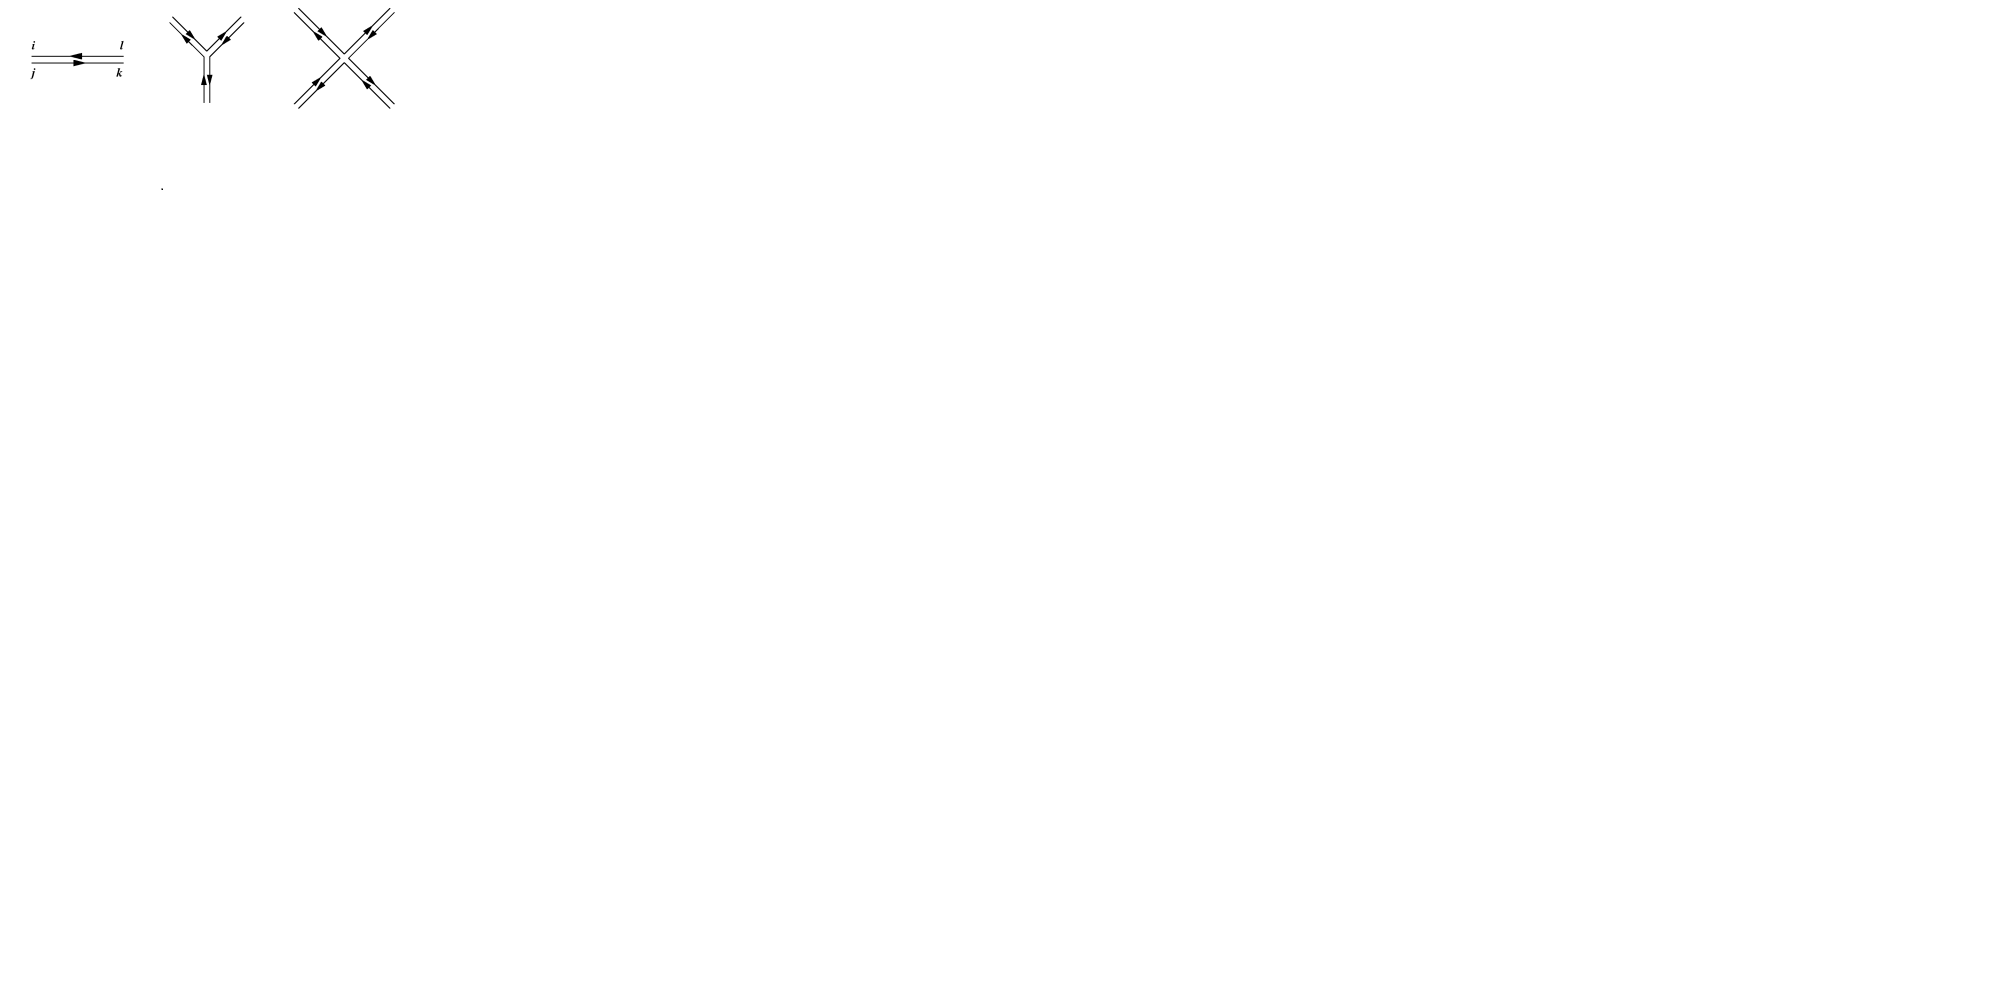
\includegraphics[scale=0.75]{double_line.png}
    \end{itemize}
\end{frame}

\begin{frame}
    \frametitle{Feynman Rules for $N\times N$ Matrix Fields (cont.)}
    \alert{$2 \to 2$ Scattering}
    \begin{itemize}
        \item[\textbullet]<2-> The contributing tree-level diagrams are given by
        \begin{center}
            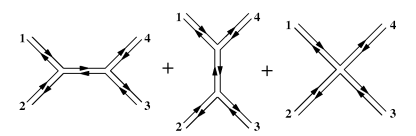
\includegraphics[scale=0.65]{tree_level.PNG}
        \end{center}
        plus all permutations of 2, 3, and 4.
        \item[\textbullet]<3-> The resulting ampluted is \[ i\mathcal{T} = \Tr[T^{a_1}T^{a_2}T^{a_3}T^{a_4}]\left(\frac{(ig)^2(-i)}{(k_1 + k_2)^2} + \frac{(ig)^2(-i)}{(k_1 + k_4)^2} - i\lambda\right) + \text{Perms} \]
    \end{itemize}
\end{frame}

\begin{frame}
    \frametitle{Feynman Rules for $N\times N$ Matrix Fields (cont.)}
    \alert{Evaluating $|\mathcal{T}|^2$}
    \begin{itemize}
        \item[\textbullet]<2-> When we square the scattering amplitude we get terms than include factors of
        \begin{itemize}
            \item[\textbullet]<3-> products of traces e.g. \[ \Tr[T^{a_{i_1}}\ldots T^{a_{i_n}}]\Tr[T^{a_{i'_1}}\ldots T^{a_{i'_n}}]^* \]
            \item[\textbullet]<4-> products of momentum factors e.g. \[ \left(\frac{g^2}{(k_{i_1}+k_{i_2})^2} + \frac{g^2}{(k_{i_3}+k_{i_4})^2} - \lambda\right)\left(\frac{g^2}{(k_{i'_1}+k_{i'_2})^2} + \frac{g^2}{(k_{i'_3}+k_{i'_4})^2} - \lambda\right) \]
        \end{itemize}
    \end{itemize}
\end{frame}

\begin{frame}
    \frametitle{Feynman Rules for $N\times N$ Matrix Fields (cont.)}
    \alert{Evaluating $|\mathcal{T}|^2$ cont.}
    \begin{itemize}
        \item[\textbullet]<2-> After summing over repeated indices, the trace products yield factors of $N^2$ and $N^4$.
        \item[\textbullet]<3-> Using momentum conservation, there are only three distinct momentum factors: 
        \begin{align*}
            A_2 &\coloneqq \frac{g^2}{(k_1 + k_4)^2} + \frac{g^2}{(k_1+k_3)^2} - \lambda \\
            A_3 &\coloneqq \frac{g^2}{(k_1 + k_2)^2} + \frac{g^2}{(k_1+k_4)^2} - \lambda \\
            A_4 &\coloneqq \frac{g^2}{(k_1 + k_3)^2} + \frac{g^2}{(k_1+k_2)^2} - \lambda 
        \end{align*}
    \end{itemize}
\end{frame}

\begin{frame}
    \frametitle{Feynman Rules for $N\times N$ Matrix Fields (cont.)}
    \alert{Evaluating $|\mathcal{T}|^2$ cont.}
    \begin{itemize}
        \item[\textbullet]<2-> The summed amplitude squared is then
        \begin{align*}
            \sum_{a_1,a_2,a_3,a_4}|\mathcal{T}|^2 &= (2N^2 + 2N^2)\sum_j |A_j|^2 + 4N^2\sum_{j\neq k} A*_jA_k \\
            &= (2N^2 - 2N^2)\sum_j |A_j|^2 + 4N^2\left(\sum_{j} A*_j\right)\left(\sum_k A_k \right)
        \end{align*}
        where $j$ and $k$ are summed over 2, 3, 4.
    \end{itemize}
\end{frame}

\begin{frame}
    \frametitle{Feynman Rules for $N\times N$ Matrix Fields (cont.)}
    \alert{Color-Ordered Feynman Rules}
    \begin{itemize}
        \item[\textbullet]<2-> To summarize, the Feynman rules for matrix fields are
        \begin{itemize}
            \item[1)]<3-> Draw the diagram in a planar fashion and number the external momenta counter-clockwise.
            \item[2)]<4-> The order of the $T^{a_i}$ in the trace is determined by the momenta numbering.
            \item[3)]<5-> Internal lines give factors of $i/k^2$.
            \item[4)]<6-> 3-point vertices give factors of $ig$. 
            \item[5)]<7-> 4-point vertices give factors of $-i\lambda$. 
        \end{itemize}
    \end{itemize}
\end{frame}

\begin{frame}
    \frametitle{Feynman Rules for $N\times N$ Matrix Fields (cont.)}
    \alert{A Complication: Tracelessness}
    \begin{itemize}
        \item[\textbullet]<2-> So far the $B$ fields have been specifically \textit{not} traceless.
        \item[\textbullet]<3-> Imposing the traceless condition is equivalent to modifying our generator product identity to be \[ (T^a)_i^{\;j}(T^a)_k^{\;l} = \delta_i^{\;l}\delta_k^{\;j} - \frac{1}{N}\delta_i^{\;j}\delta_k^{\;l} \]
        \item[\textbullet]<4-> This would seem to again make computations more involved, but we will see that this winds up not being the case.
    \end{itemize}
\end{frame}

\begin{frame}
    \frametitle{The Twister Formalism}
    \alert{Let's Do the Twist!}
    \begin{itemize}
        \item[\textbullet]<2-> Recall that calculations in spinor electrodynamics for massless fermions can be greatly simplified by introducing the notation of \textit{twistors}:\[ |p] \coloneqq u_-(p) = v_+(p); \quad [p| \coloneqq \bar{u}_+(p) = \bar{v}_-(p) \] \[ \bra{p} \coloneqq u_+(p) = v_-(p); \quad \bra{p} \coloneqq \bar{u}_-(p) = \bar{v}_+(p) \]
        \item[\textbullet]<3-> We can also express boson polarization vectors (with respect to an arbitrary reference momentum $q$) in twistor notation: \[ \epsilon_+^\mu(k;q) = -\frac{\bra{q}\gamma^\mu|k]}{\sqrt{2}\ev{qk}}; \quad \epsilon_-^\mu(k;q) = -\frac{[q|\gamma^\mu\bra{k}}{\sqrt{2}[qk]} \]
    \end{itemize}
\end{frame}

\begin{frame}
    \frametitle{The Twister Formalism (cont.)}
    \alert{Polarization Twister Dot Products}
    \begin{itemize}
        \item[\textbullet]<2-> We will need to express the dot products of polarization vectors in terms of their twister representations.
        \item[\textbullet]<3-> The necessare equations are
        \begin{align*}
            \epsilon_+(k;q)\cdot\epsilon_+(k';q') &= \frac{\ev{qq'}[kk']}{\ev{qk}\ev{q'k'}} \\
            \epsilon_-(k;q)\cdot\epsilon_-(k';q') &= \frac{[qq']\ev{kk'}}{[qk][q'k']} \\
            \epsilon_+(k;q)\cdot\epsilon_-(k';q') &= \frac{\ev{qk'}[kq']}{\ev{qk}[q'k']}
        \end{align*} 
    \end{itemize}
\end{frame}

\begin{frame}
    \frametitle{Helicity Convention}
    \alert{Simplifying the Twister/Helicty Connection}
    \begin{itemize}
        \item[\textbullet]<2-> Assign all external lines of a vertex outgoing momenta $k_i$.
        \begin{itemize}
            \item[\textbullet]<3-> A particle with assigned momentum $p$ has physical momentum $\epsilon_p p$ where \[ \epsilon_p = \begin{cases} +1 & \text{for physically outgoing particles} \\ -1 & \text{for physically incomming particles} \end{cases} \]
        \end{itemize}
        \item[\textbullet]<4-> With this convention, 
        \begin{itemize}
            \item[\textbullet]<5-> $|p]$ and $[p|$ twistors correspond to particles with positive helicity.
            \item[\textbullet]<6-> $\ket{p}$ and $\bra{p}$ twistors correspond to particles with negative helicity. 
        \end{itemize}
    \end{itemize}
\end{frame}

\begin{frame}
    \frametitle{Tree-Level $N$-Gluon Scattering}
    \alert{Back to Amplitudes}
    \begin{itemize}
        \item[\textbullet]<2-> We return now to the lagrangian for $SU(N)$ Yang-Mills theory in Gervais-Neveu gauge: \[ \mathcal{L} = \Tr[-\frac{1}{2}\partial^\mu A^\nu \partial_\mu A_\nu - i\sqrt{2}g\partial^\mu A^\nu A_\nu A_\mu + \frac{1}{4}g^2 A^\mu A^\nu A_\mu A_\nu] \]
        \item[\textbullet]<3-> The tree-level n-gluon scattering amplitude may be written as \[ \mathcal{T} = g^{n-2}\sum_{\pi\in\tilde{S}_n} \Tr[T^{a_{\pi_1}}\ldots T^{a_{\pi_n}}]A(\pi_1,\ldots,\pi_n) \] where the sum is over all non-cyclic permutations of $n$ elements, and the $A()$ are \textit{partial amplitudes} that are computed with the color-ordered Feynman rules. 
    \end{itemize}
\end{frame}

\begin{frame}
    \frametitle{Tree-Level $N$-Gluon Scattering (cont.)}
    \alert{The Partial Amplitudes}
    \begin{itemize}
        \item[\textbullet]<2-> The partial amplitudes possess three useful symmetries:
        \begin{itemize}
            \item[1)]<3-> Cyclic symmetry: \[A(2,\ldots,n,1) = A(1,2,\ldots,n) \]
            \item[2)]<4-> Reflection symmetry: \[ A(n,\ldots,2,1) = (-1)^nA(1,2,\ldots,n) \]
            \item[3)]<5-> ``The Third Symmetry'': \[ A(1,2,3,4) = -A(1,2,4,3) - A(1,4,2,3) \]
        \end{itemize}
    \end{itemize}
\end{frame}

\begin{frame}
    \frametitle{Tree-Level $N$-Gluon Scattering (cont.)}
    \alert{Applying the Twistor Formalism}
    \begin{itemize}
        \item[\textbullet]<2-> Looking at our lagrangian, we can deduce our propagator and vertex factors:
        \begin{itemize}
            \item<3-> \[ \tilde{\Delta}_{\mu\nu} = \frac{g_{\mu\nu}}{k^2 - i\epsilon} \]
            \item<4-> \[ iV_{\mu\nu\rho}(p,q,r) = -i\sqrt{2}g(p_\rho g_{\mu\nu} + q_\mu g_{\nu\rho} + r_\nu g_{\rho\mu}) \]
            \item<5-> \[ iV_{\mu\nu\rho\sigma} = ig^2 g_{\mu\rho}g_{\nu\sigma} \]   
        \end{itemize}
    \end{itemize}
\end{frame}

\begin{frame}
    \frametitle{Tree-Level $N$-Gluon Scattering (cont.)}
    \alert{Applying the Twistor Formalism (cont.)}
    \begin{itemize}
        \item[\textbullet]<2-> To apply the twister formalism, we contract momenta with the corresponding polarization vector.
        \item[\textbullet]<3-> The vertex factors then become 
        \begin{itemize}
            \item<4-> \[ iV_{123} = -i\sqrt{2}g\left[(\epsilon_1\epsilon_3) + (\epsilon_2\epsilon_3)(k_2\epsilon_1) + (\epsilon_3\epsilon_1)(k_3\epsilon_2)\right] \]
            \item<5-> \[ iV_{1234} = +ig^2(\epsilon_1\epsilon_3)(\epsilon_2\epsilon_4) \]  
        \end{itemize}
        \item[\textbullet]<6-> Clearly, our calculations will be vastly simplified if we can get the majority of these polarization dot products to vanish, and we will see that is in fact easily achievable.
    \end{itemize}
\end{frame}

\begin{frame}
    \frametitle{Tree-Level $N$-Gluon Scattering (cont.)}
    \alert{A Condition on Helicities}
    \begin{itemize}
        \item[\textbullet]<2-> With some simple edge/vertex counting, we can see that every term in the final amplitude will contain at least one product betwen polarization vectors.
        \item[\textbullet]<3-> Becuase the polarization vectors are transverse, this restricts the possible combinations of helicities that can have non-zero partial amplitudes.
        \item[\textbullet]<4-> Specifically, if all, or all but one, of the external gluons have the same helicity, the amplitude is zero, i.e. \[ A(1^\pm, 2^+, \ldots, n^+) = A(1^\pm, 2^-, \ldots, n^-) = 0 \] 
    \end{itemize}
\end{frame}

\begin{frame}
    \frametitle{Tree-Level $N$-Gluon Scattering (cont.)}
    \alert{Calculating a Partial Amplitude}
    \begin{itemize}
        \item[\textbullet]<2-> Consider the partial amplitude $A(1^-, 2^-, 3^+, 4^+)$, given by the diagrams
        \begin{center}
            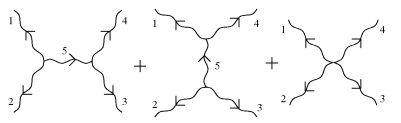
\includegraphics[scale=0.65]{partial_amp_dia.PNG}
        \end{center}
        \item[\textbullet]<3-> Choosing our reference momenta to be $q_1 = q_2 = k_3$ and $q_3 = q_4 = k_2$ causes all polarization products to vannish except for \[ \epsilon_1\cdot\epsilon_4 = \frac{\ev{21}[43]}{\ev{24}[31]} \]
    \end{itemize}
\end{frame}

\begin{frame}
    \frametitle{Tree-Level $N$-Gluon Scattering (cont.)}
    \alert{Calculating a Partial Amplitude (cont.)}
    \begin{itemize}
        \item[\textbullet]<2-> Our choice of reference momenta causes both the second and third diagrams in the previous slide to vanish.
        \item[\textbullet]<3-> Evaluating the remaining diagram, we have
        \item<4-> $ iV_{125} = -i\sqrt{2}g\left[(\epsilon_1\epsilon_2)(k_1\epsilon_5) + (\epsilon_2\epsilon_5)(k_2\epsilon_1) + (\epsilon_5\epsilon_1)(k_5\epsilon_2)\right] $
        \item<5-> $ iV_{345'} = -i\sqrt{2}g\left[(\epsilon_3\epsilon_4)(k_3\epsilon_5) + (\epsilon_4\epsilon_5)(k_4\epsilon_3) + (\epsilon_5\epsilon_3)(k_{5'}\epsilon_4)\right] $
        \item[\textbullet]<6-> Note that $\epsilon_5$ is just a placeholder for the internal propagator, and $k_{5'} = -k_5$.
        \item[\textbullet]<7-> After substituting in the propagator and take the product of these vertex factors, only one term winds up being nonvanishing, giving \[ ig^2A(1^-,2^-,3^+,4^+) = (-i\sqrt{2}g)^2(i/s_{12})(\epsilon_1\epsilon_4)(k_5\epsilon_2)(k_4\epsilon_3) \] where $s_{12} = -(k_1 + k_2)^2 = \ev{12}[21]$.
    \end{itemize}
\end{frame}

\begin{frame}
    \frametitle{Tree-Level $N$-Gluon Scattering (cont.)}
    \alert{Plugging in the Twistors}
    \begin{itemize}
        \item[\textbullet]<2-> Using the twistor expressions for the dot product of a momentum and a poloarization vector \[ p\cdot\epsilon_+(k;q) = \frac{\ev{qp}[pk]}{\sqrt{2}[qk]}; \quad p\cdot\epsilon_-(k;q) = \frac{[qp]\ev{pk}}{\sqrt{2}[qk]}, \]
        \item[\textbullet]<3-> we can now express our partial amplitude as \[ A(1^-, 2^-, 3^+, 4^+) = \frac{\ev{21}[43]^2}{[21][32]\ev{23}} = \frac{\ev{12}^4}{\ev{12}\ev{23}\ev{34}\ev{41}} \]
        \item[\textbullet]<4-> Note that this is a specific case of the \textit{Parke-Taylor Maximum Helicity Violoating} amplitudes: \[ A(1^+\ldots i^-\ldots j^-\ldots n^+) \propto \frac{\ev{ij}^4}{\ev{12}\ev{23}\cdots\ev{(n-1)n}\ev{n1}} \]
        \end{itemize}
\end{frame}

\begin{frame}
    \frametitle{Tree-Level $N$-Gluon Scattering (cont.)}
    \alert{The Other Partial Amplitudes}
    \begin{itemize}
        \item[\textbullet]<2-> We can now use the cyclic symmetry of the partial amplitudes to get any other amplitude in which the helicities with the same sign sit next to each other (e.g. $A(1^-,2^+,3^+,4^-)$).
        \item[\textbullet]<3-> Amplitudes with alternating helicities can be obtained using ``the third symmetry'' (e.g. $A(1^+,2^-,3^+,4^-)$).
        \item[\textbullet]<4-> The only distinct amplitudes that must be calculated may be denoted \[ A_2 \coloneqq A(1,4,2,3); \; A_3 \coloneqq A(1,2,3,4); \; A_4 \coloneqq A(1,4,3,2) \]  
    \end{itemize}
\end{frame}

\begin{frame}
    \frametitle{Tree-Level $N$-Gluon Scattering (cont.)}
    \alert{Color Summing}
    \begin{itemize}
        \item[\textbullet]<2-> We are now ready to apply our results for matrix fields to calcualte the color summed squared amplitude.
        \item[\textbullet]<3-> The ``third symmetry'' implies that $\sum_jA_j$ vanishes, so our expression simplifies to \[ \sum_{\text{colors}}|\mathcal{T}|^2 = 2N^2(N^2 - 1)g^4\left(|A_2|^2 + |A_3|^2 + |A_4|^2\right) \]
        \item[\textbullet]<4-> If we take gluons 1 and 2 to be incoming, and 3 and 4 outgoing, we can express this in terms of the usual Mandelstam variables: \[ \sum_{\text{colors}}|\mathcal{T}|^2 = 2N^2(N^2 - 1)g^4s^4\left(\frac{1}{s^2t^2} + \frac{1}{t^2u^2} + \frac{1}{u^2s^2}\right) \]
    \end{itemize}
\end{frame}

\begin{frame}
    \frametitle{Tree-Level $N$-Gluon Scattering (cont.)}
    \alert{Full Spin/Color Sum/Average}
    \begin{itemize}
        \item[\textbullet]<2-> Finally, we can sum over helicities as well.
        \item[\textbullet]<3-> Of course, we want to average over initial colors/helicities, so we must divide by a factor of $4(N^2 - 1)^2$.
        \item[\textbullet]<4-> Our final result is then \[ \boxed{\sum_{\substack{\text{colors}\\\text{helicities}}} |\mathcal{T}|^2 = \frac{N^2}{N^2 - 1}g^4(s^4 + t^4 + u^4)\left(\frac{1}{s^2t^2} + \frac{1}{t^2u^2} + \frac{1}{u^2s^2}\right) } \] 
    \end{itemize}
\end{frame}

\end{document}